\chapter{Additional Figures}
\label{chap:additional_figs}

%%%%%%%%%%%%%%%%%%%%%%%%%%%%%%%%%%%%%%%%%%%%%%%%%%%%%%%%%%%%%%%%%%%%%%%%%%%%%%%%
\section{netgain}

\begin{figure}[H]
\begin{centering}
\begin{singlespace}
    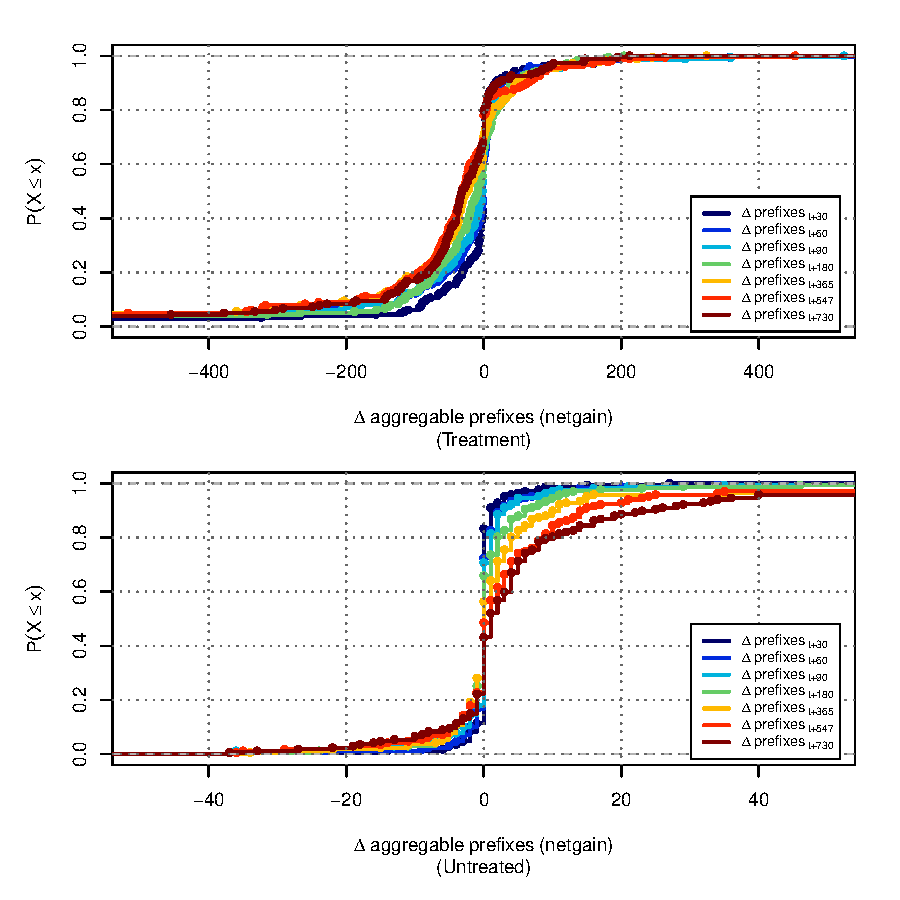
\includegraphics[width=6in]{figures/behavior-netgain-1998_2001-corr.pdf}
    \vspace{-2em}\\
    \caption{Cumulative distribution function of change in number ofaggregable prefixes (netgain) advertised by treated and untreated(control) ASes, for the period 1998--2001.}
\end{singlespace}
\end{centering}
\end{figure}
\begin{figure}[H]
\begin{centering}
\begin{singlespace}
    \includegraphics[width=6in]{figures/behavior-netgain-2001_2004-corr.pdf}
    \vspace{-2em}\\
    \caption{Cumulative distribution function of change in number ofaggregable prefixes (netgain) advertised by treated and untreated(control) ASes, for the period 2001--2004.}
\end{singlespace}
\end{centering}
\end{figure}
\begin{figure}[H]
\begin{centering}
\begin{singlespace}
    \includegraphics[width=6in]{figures/behavior-netgain-2004_2007-corr.pdf}
    \vspace{-2em}\\
    \caption{Cumulative distribution function of change in number ofaggregable prefixes (netgain) advertised by treated and untreated(control) ASes, for the period 2004--2007.}
\end{singlespace}
\end{centering}
\end{figure}
\begin{figure}[H]
\begin{centering}
\begin{singlespace}
    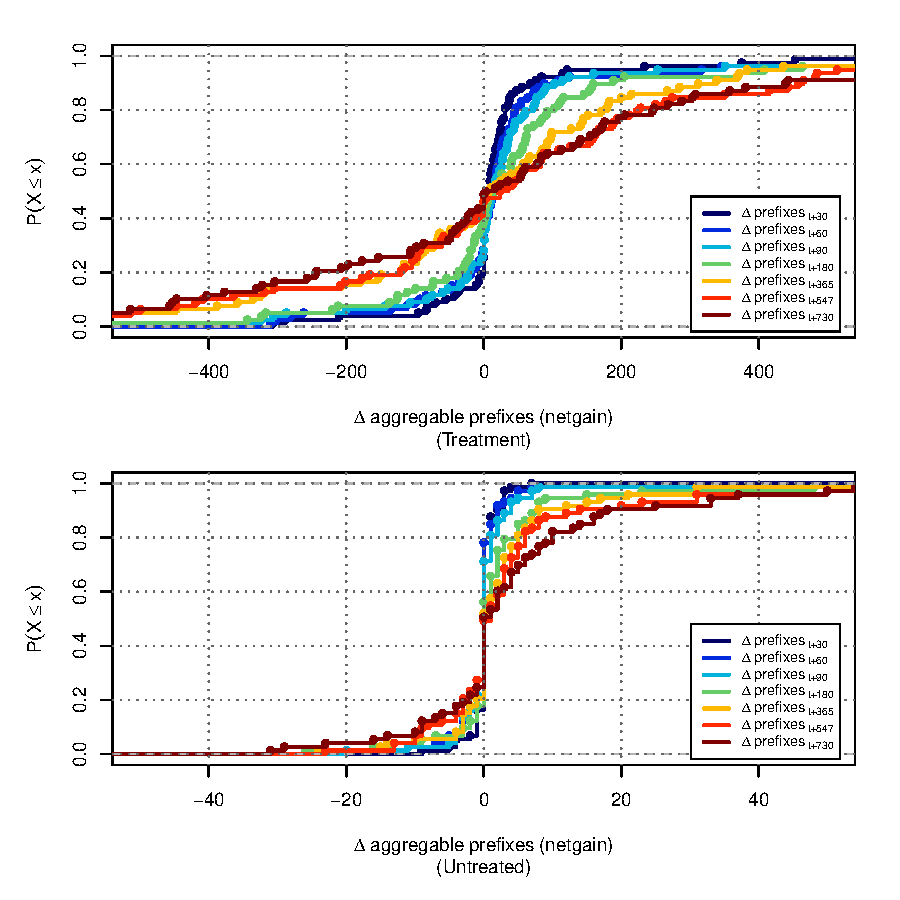
\includegraphics[width=6in]{figures/behavior-netgain-2007_2010-corr.pdf}
    \vspace{-2em}\\
    \caption{Cumulative distribution function of change in number ofaggregable prefixes (netgain) advertised by treated and untreated(control) ASes, for the period 2007--2010.}
\end{singlespace}
\end{centering}
\end{figure}

%%%%%%%%%%%%%%%%%%%%%%%%%%%%%%%%%%%%%%%%%%%%%%%%%%%%%%%%%%%%%%%%%%%%%%%%%%%%%%%%
\section{Relative netgain}

\[
\textrm{relative netgain} = \frac{\textrm{netgain}_{t+k}}
                                 {\textrm{netgain}_{t+0}}, k > 0
\]

\begin{figure}[H]
\begin{centering}
\begin{singlespace}
    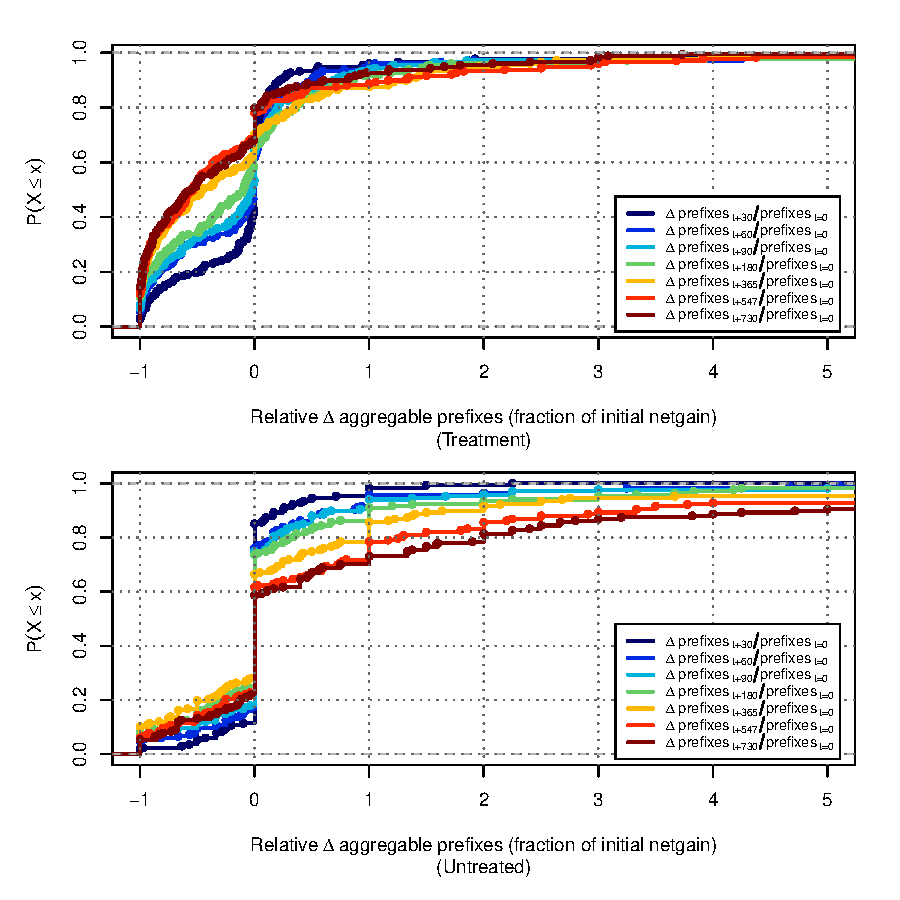
\includegraphics[width=6in]{figures/behavior-rel_netgain-1998_2001-corr.pdf}
    \vspace{-2em}\\
    \caption{Cumulative distribution function of relative change in number of aggregable prefixes (netgain) advertised by treated and untreated (control) ASes, for the period 1998--2001.}
\end{singlespace}
\end{centering}
\end{figure}
\begin{figure}[H]
\begin{centering}
\begin{singlespace}
    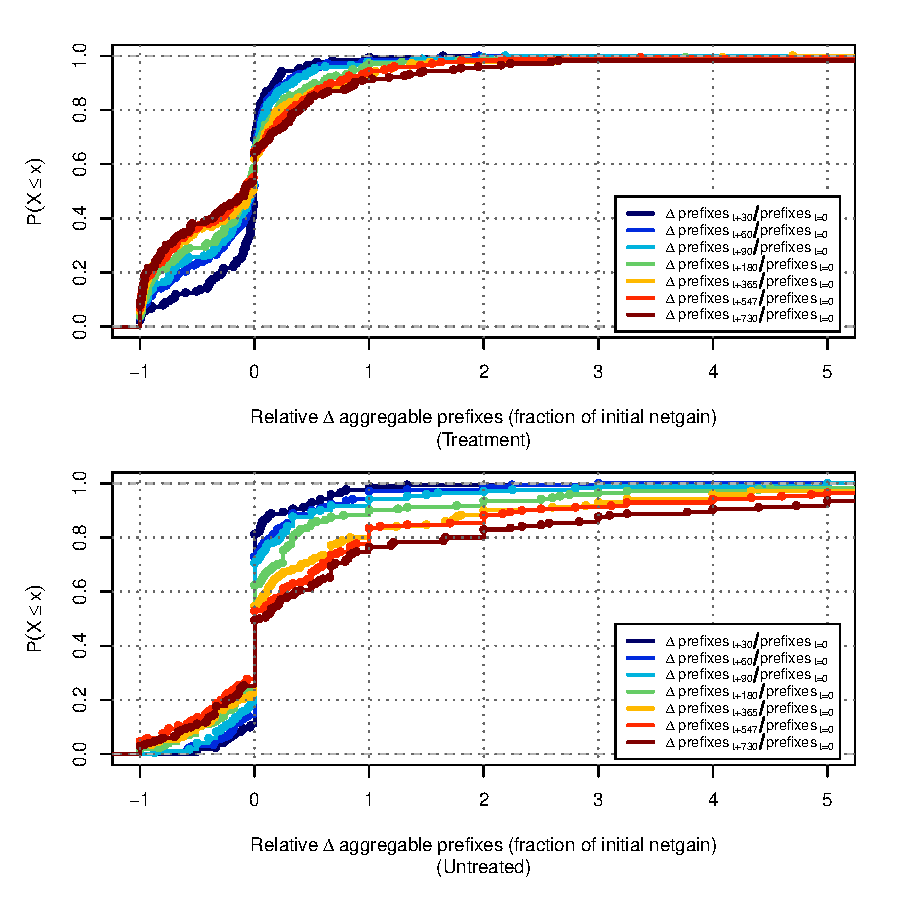
\includegraphics[width=6in]{figures/behavior-rel_netgain-2001_2004-corr.pdf}
    \vspace{-2em}\\
    \caption{Cumulative distribution function of relative change in number of aggregable prefixes (netgain) advertised by treated and untreated (control) ASes, for the period 2001--2004.}
\end{singlespace}
\end{centering}
\end{figure}
\begin{figure}[H]
\begin{centering}
\begin{singlespace}
    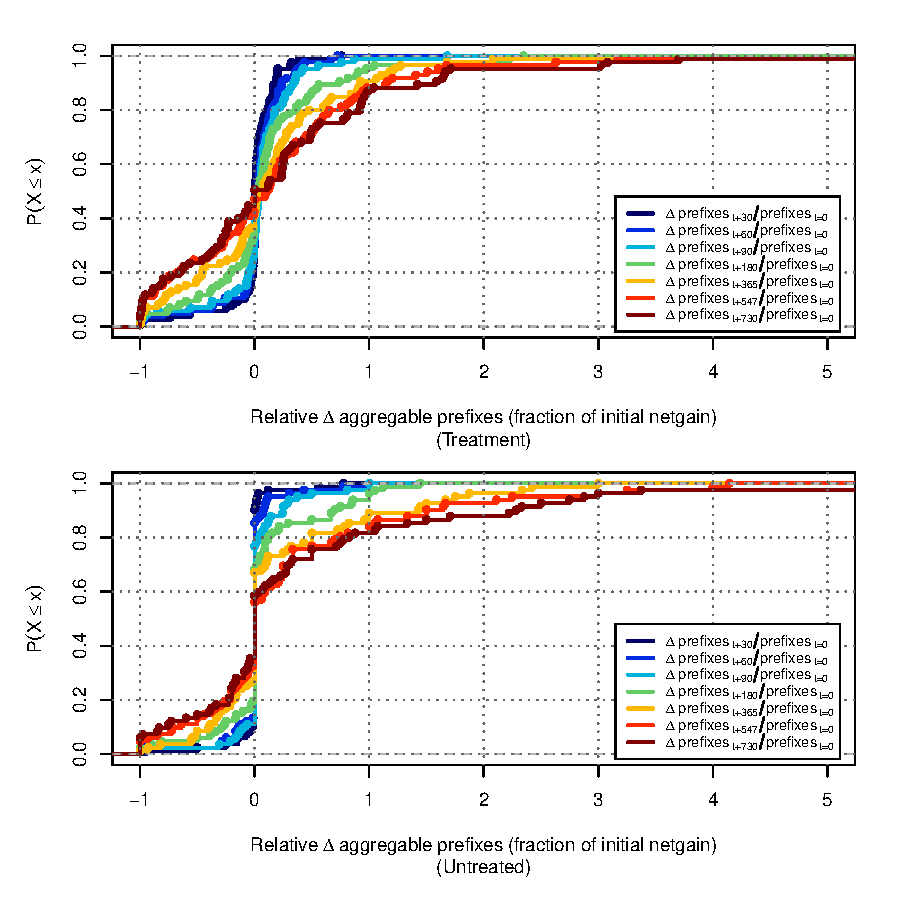
\includegraphics[width=6in]{figures/behavior-rel_netgain-2004_2007-corr.pdf}
    \vspace{-2em}\\
    \caption{Cumulative distribution function of relative change in number of aggregable prefixes (netgain) advertised by treated and untreated (control) ASes, for the period 2004--2007.}
\end{singlespace}
\end{centering}
\end{figure}
\begin{figure}[H]
\begin{centering}
\begin{singlespace}
    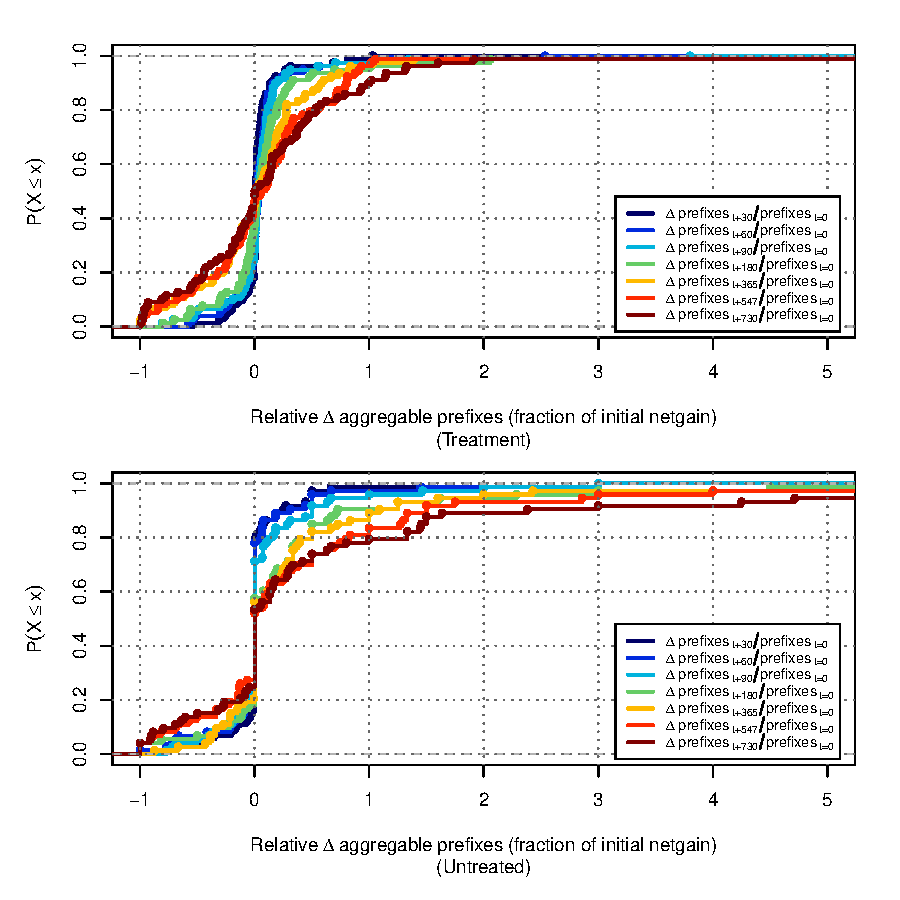
\includegraphics[width=6in]{figures/behavior-rel_netgain-2007_2010-corr.pdf}
    \vspace{-2em}\\
    \caption{Cumulative distribution function of relative change in number of aggregable prefixes (netgain) advertised by treated and untreated (control) ASes, for the period 2007--2010.}
\end{singlespace}
\end{centering}
\end{figure}

%%%%%%%%%%%%%%%%%%%%%%%%%%%%%%%%%%%%%%%%%%%%%%%%%%%%%%%%%%%%%%%%%%%%%%%%%%%%%%%%
\section{netsnow}

\begin{figure}[H]
\begin{centering}
\begin{singlespace}
    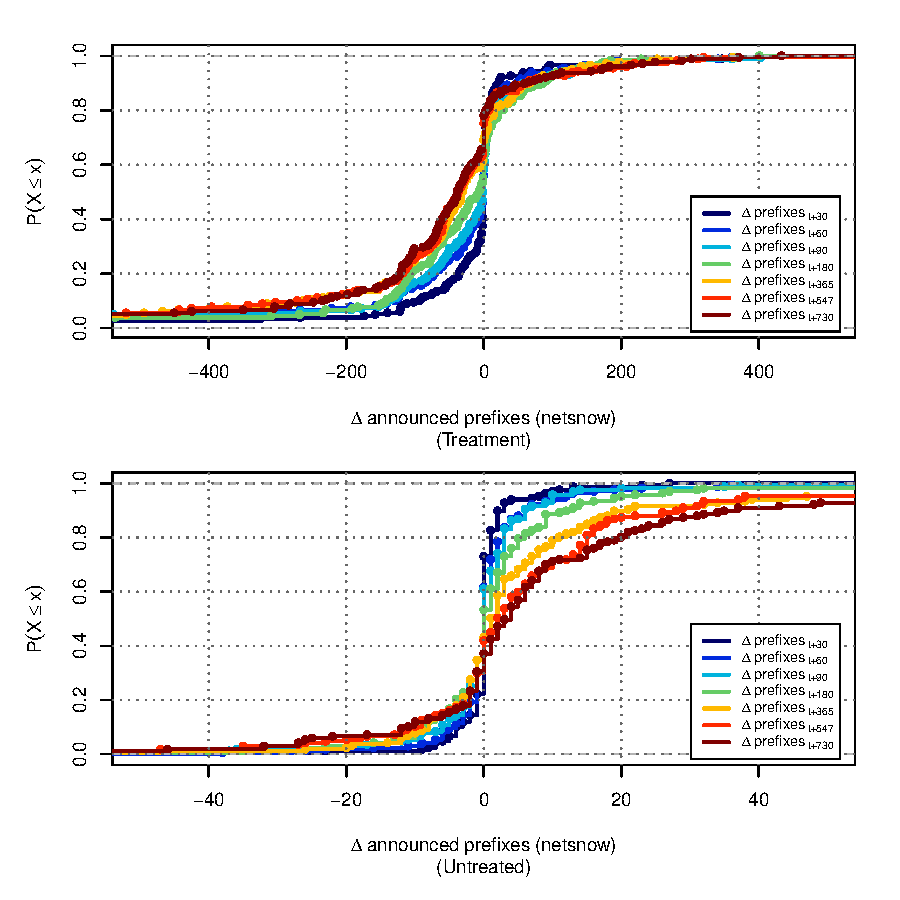
\includegraphics[width=6in]{figures/behavior-netsnow-1998_2001-corr.pdf}
    \vspace{-2em}\\
    \caption{Cumulative distribution function of change in total number of prefixes (netsnow) advertised by treated and untreated (control) ASes, for the period 1998--2001.}
\end{singlespace}
\end{centering}
\end{figure}
\begin{figure}[H]
\begin{centering}
\begin{singlespace}
    \includegraphics[width=6in]{figures/behavior-netsnow-2001_2004-corr.pdf}
    \vspace{-2em}\\
    \caption{Cumulative distribution function of change in total number of prefixes (netsnow) advertised by treated and untreated (control) ASes, for the period 2001--2004.}
\end{singlespace}
\end{centering}
\end{figure}
\begin{figure}[H]
\begin{centering}
\begin{singlespace}
    \includegraphics[width=6in]{figures/behavior-netsnow-2004_2007-corr.pdf}
    \vspace{-2em}\\
    \caption{Cumulative distribution function of change in total number of prefixes (netsnow) advertised by treated and untreated (control) ASes, for the period 2004--2007.}
\end{singlespace}
\end{centering}
\end{figure}
\begin{figure}[H]
\begin{centering}
\begin{singlespace}
    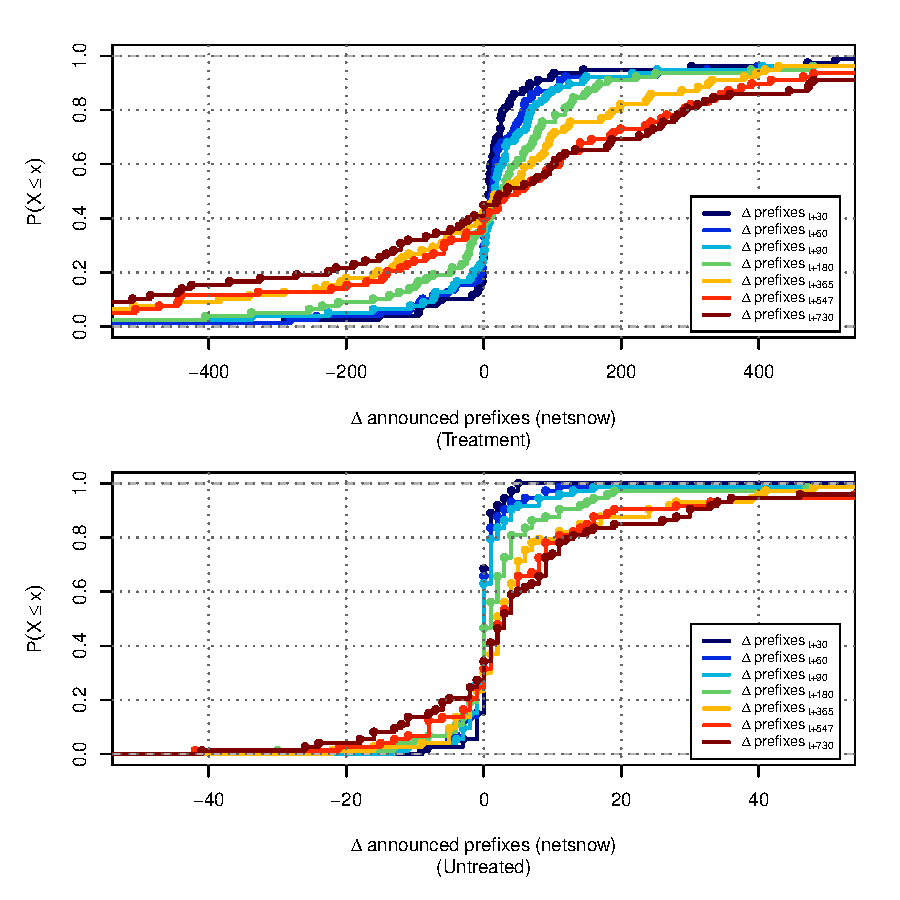
\includegraphics[width=6in]{figures/behavior-netsnow-2007_2010-corr.pdf}
    \vspace{-2em}\\
    \caption{Cumulative distribution function of change in total number of prefixes (netsnow) advertised by treated and untreated (control) ASes, for the period 2007--2010.}
\end{singlespace}
\end{centering}
\end{figure}

%%%%%%%%%%%%%%%%%%%%%%%%%%%%%%%%%%%%%%%%%%%%%%%%%%%%%%%%%%%%%%%%%%%%%%%%%%%%%%%%
\section{Relative netsnow}

\[
\textrm{relative netsnow} = \frac{\textrm{netsnow}_{t+k}}
                                 {\textrm{netsnow}_{t+0}}, k > 0
\]

\begin{figure}[H]
\begin{centering}
\begin{singlespace}
    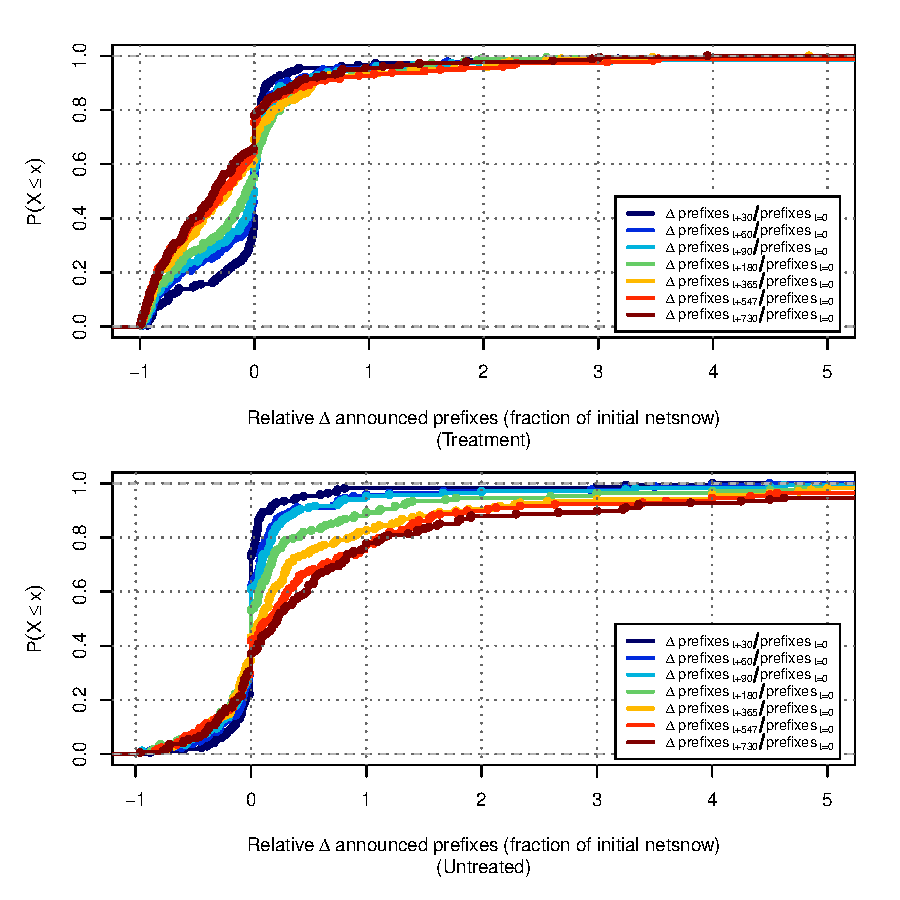
\includegraphics[width=6in]{figures/behavior-rel_netsnow-1998_2001-corr.pdf}
    \vspace{-2em}\\
    \caption{Cumulative distribution function of relative change in total number of prefixes (netsnow) advertised by treated and untreated (control) ASes, for the period 1998--2001.}
\end{singlespace}
\end{centering}
\end{figure}
\begin{figure}[H]
\begin{centering}
\begin{singlespace}
    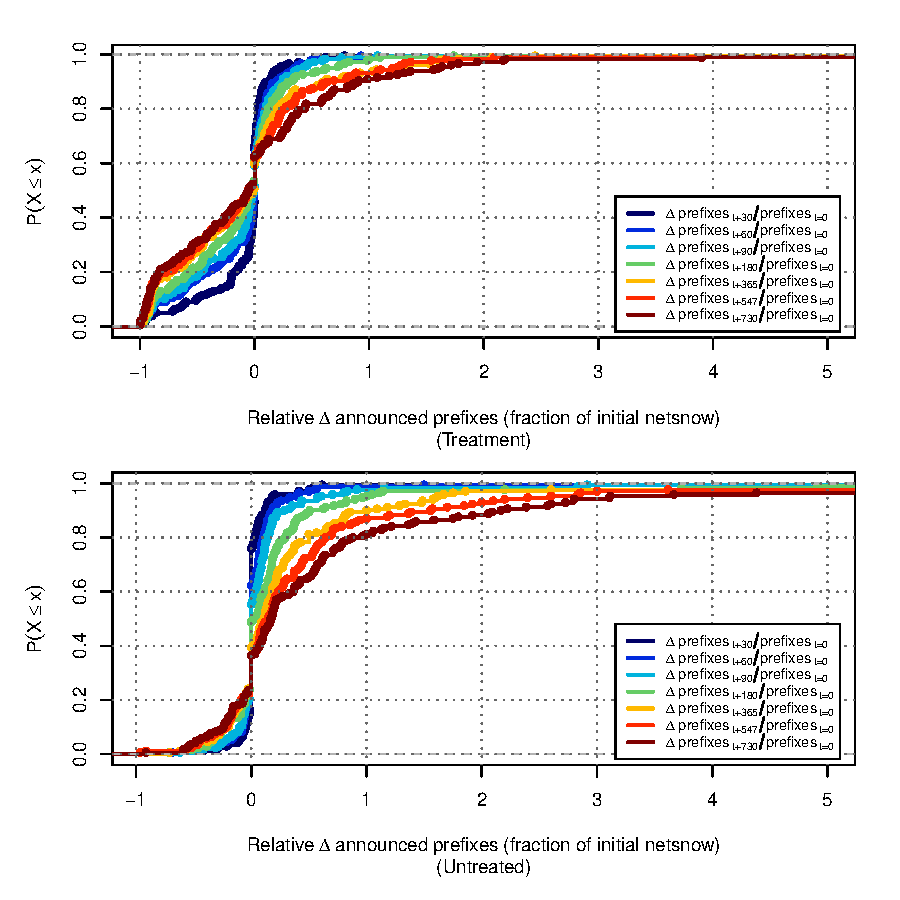
\includegraphics[width=6in]{figures/behavior-rel_netsnow-2001_2004-corr.pdf}
    \vspace{-2em}\\
    \caption{Cumulative distribution function of relative change in total number of prefixes (netsnow) advertised by treated and untreated (control) ASes, for the period 2001--2004.}
\end{singlespace}
\end{centering}
\end{figure}
\begin{figure}[H]
\begin{centering}
\begin{singlespace}
    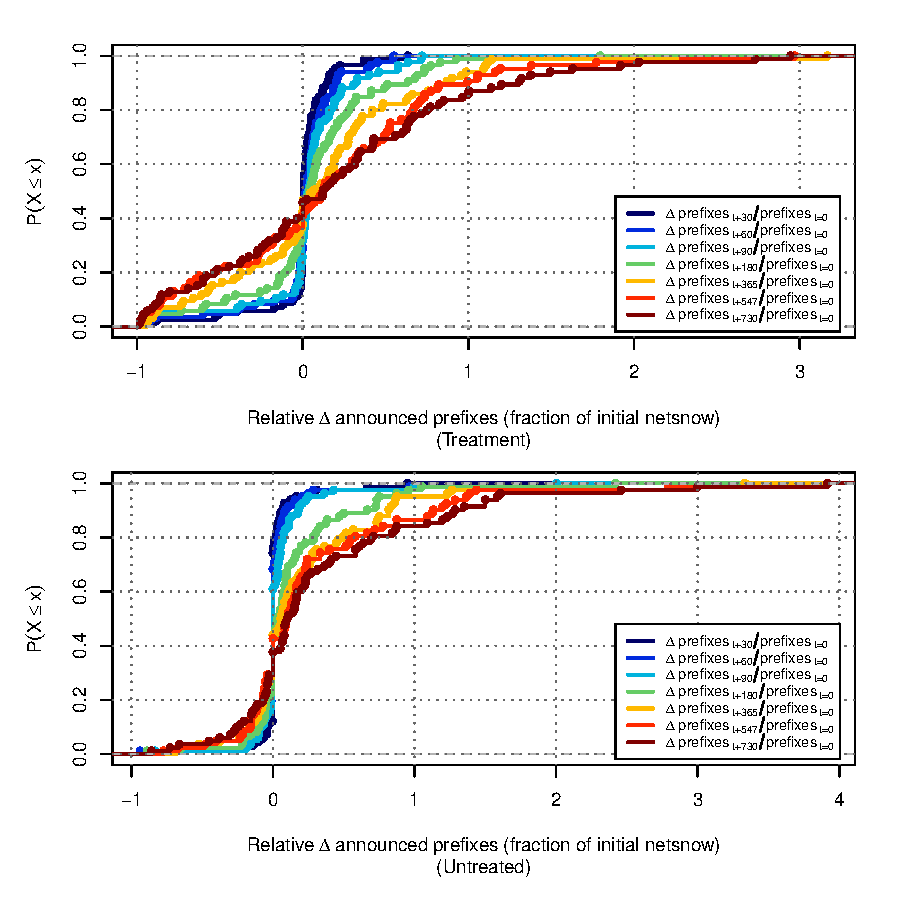
\includegraphics[width=6in]{figures/behavior-rel_netsnow-2004_2007-corr.pdf}
    \vspace{-2em}\\
    \caption{Cumulative distribution function of relative change in total number of prefixes (netsnow) advertised by treated and untreated (control) ASes, for the period 2004--2007.}
\end{singlespace}
\end{centering}
\end{figure}
\begin{figure}[H]
\begin{centering}
\begin{singlespace}
    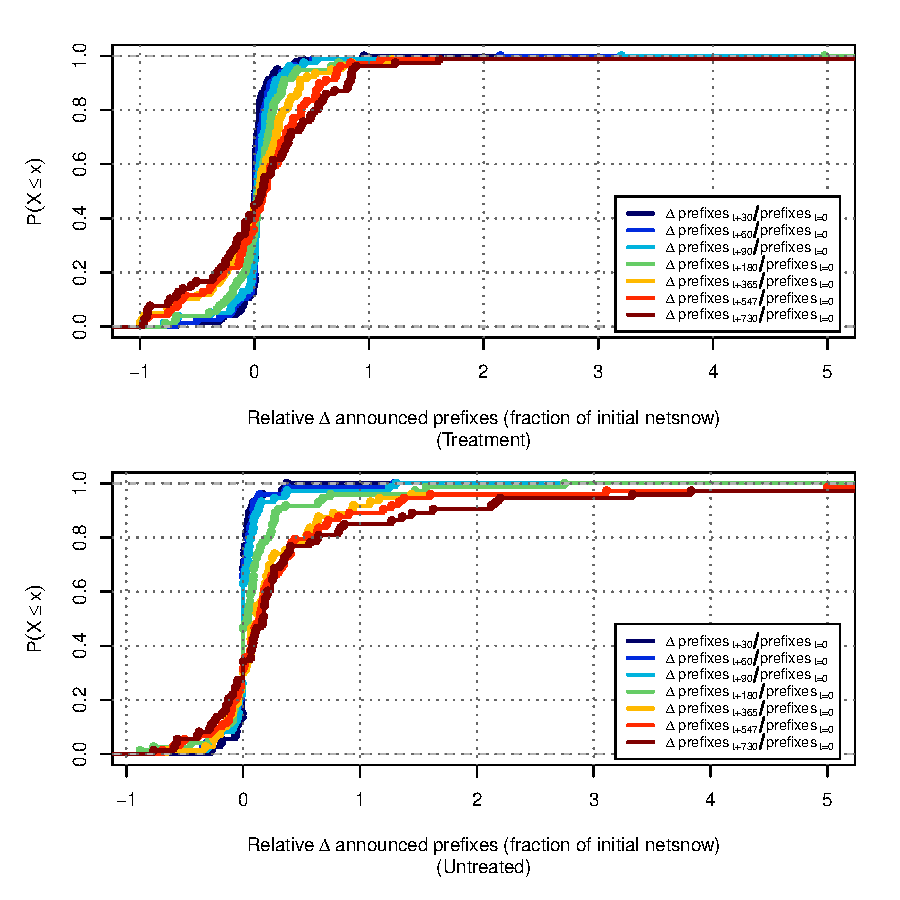
\includegraphics[width=6in]{figures/behavior-rel_netsnow-2007_2010-corr.pdf}
    \vspace{-2em}\\
    \caption{Cumulative distribution function of relative change in total number of prefixes (netsnow) advertised by treated and untreated (control) ASes, for the period 2007--2010.}
\end{singlespace}
\end{centering}
\end{figure}

%%%%%%%%%%%%%%%%%%%%%%%%%%%%%%%%%%%%%%%%%%%%%%%%%%%%%%%%%%%%%%%%%%%%%%%%%%%%%%%%
\section{Fraction Aggregable}

\[
\textrm{fraction aggregable} = \frac{\textrm{netgain}_{t+k}}
                                    {\textrm{netsnow}_{t+k}}
\]

\begin{figure}[H]
\begin{centering}
\begin{singlespace}
    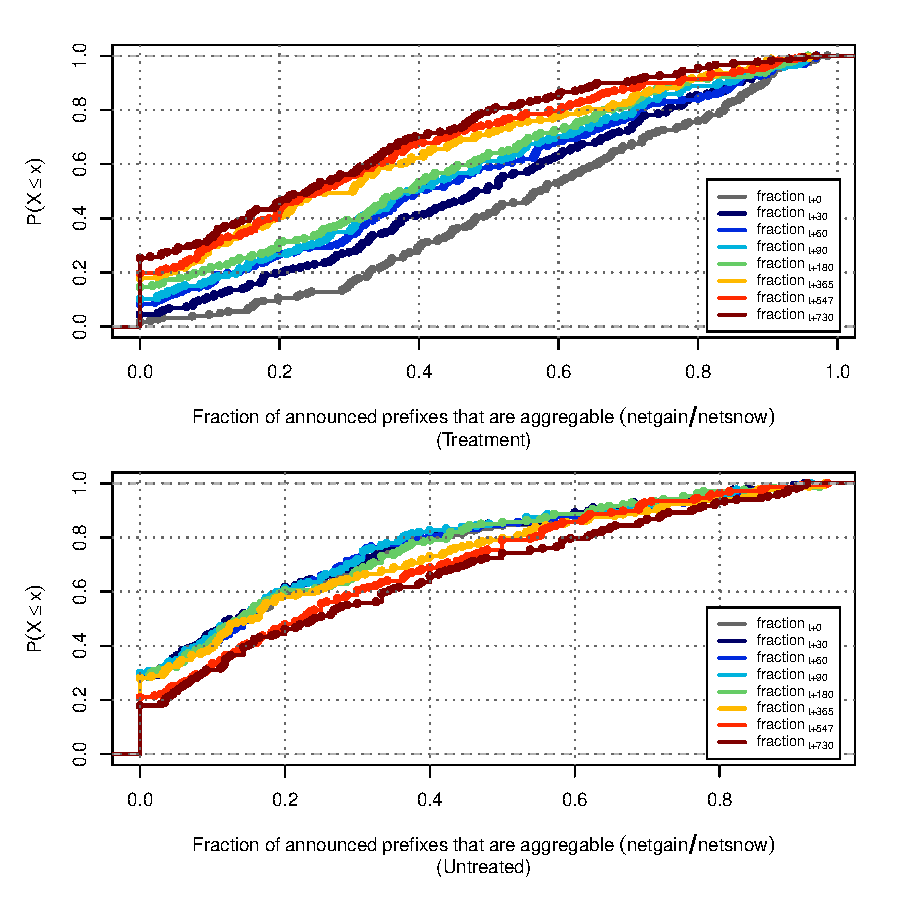
\includegraphics[width=6in]{figures/behavior-frac_deagg-1998_2001-corr.pdf}
    \vspace{-2em}\\
    \caption{Cumulative distribution function of change in the fraction of prefixes advertised by treated and untreated (control) ASes that can be aggregated without affecting routing policy, for the period 1998--2001.}
\end{singlespace}
\end{centering}
\end{figure}
\begin{figure}[H]
\begin{centering}
\begin{singlespace}
    \includegraphics[width=6in]{figures/behavior-frac_deagg-2001_2004-corr.pdf}
    \vspace{-2em}\\
    \caption{Cumulative distribution function of change in the fraction of prefixes advertised by treated and untreated (control) ASes that can be aggregated without affecting routing policy, for the period 2001--2004.}
\end{singlespace}
\end{centering}
\end{figure}
\begin{figure}[H]
\begin{centering}
\begin{singlespace}
    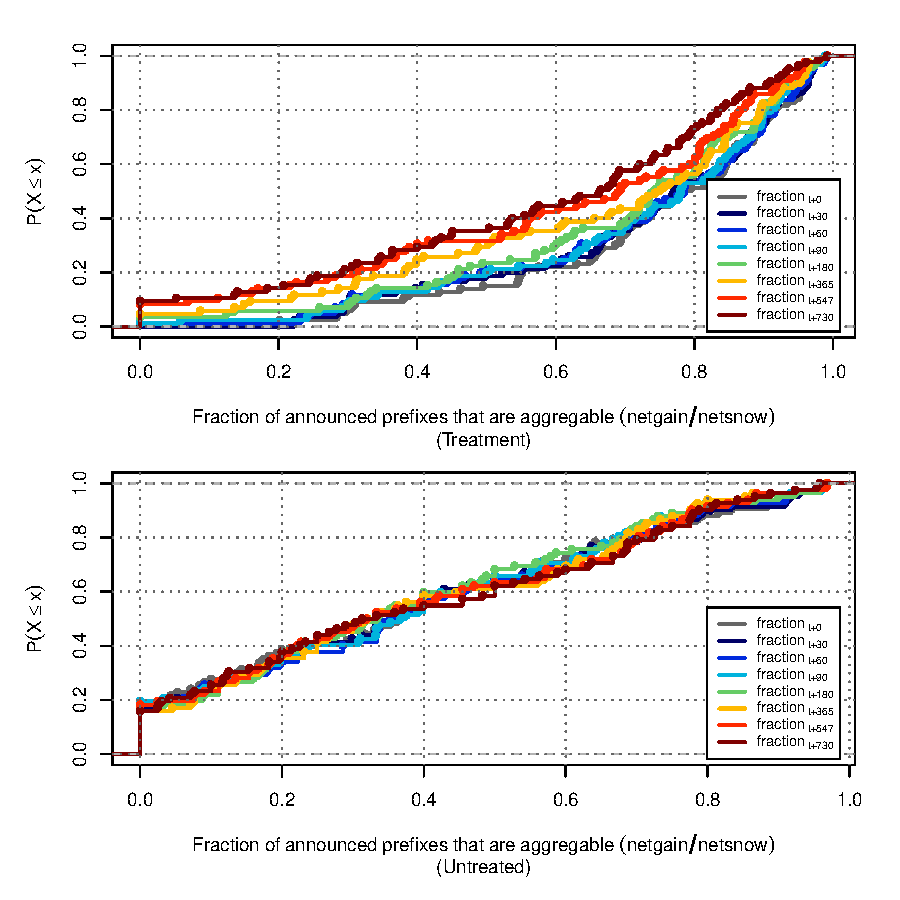
\includegraphics[width=6in]{figures/behavior-frac_deagg-2004_2007-corr.pdf}
    \vspace{-2em}\\
    \caption{Cumulative distribution function of change in the fraction of prefixes advertised by treated and untreated (control) ASes that can be aggregated without affecting routing policy, for the period 2004--2007.}
\end{singlespace}
\end{centering}
\end{figure}
\begin{figure}[H]
\begin{centering}
\begin{singlespace}
    \includegraphics[width=6in]{figures/behavior-frac_deagg-2007_2010-corr.pdf}
    \vspace{-2em}\\
    \caption{Cumulative distribution function of change in the fraction of prefixes advertised by treated and untreated (control) ASes that can be aggregated without affecting routing policy, for the period 2007--2010.}
\end{singlespace}
\end{centering}
\end{figure}

%%%%%%%%%%%%%%%%%%%%%%%%%%%%%%%%%%%%%%%%%%%%%%%%%%%%%%%%%%%%%%%%%%%%%%%%%%%%%%%%
\section{Deaggregation Factor}

\[
\textrm{fraction aggregable} = \frac{\textrm{netsnow}_{t+k}}
                            {\textrm{netsnow}_{t+k} - \textrm{netgain}_{t+k}}
\]

\begin{figure}[H]
\begin{centering}
\begin{singlespace}
    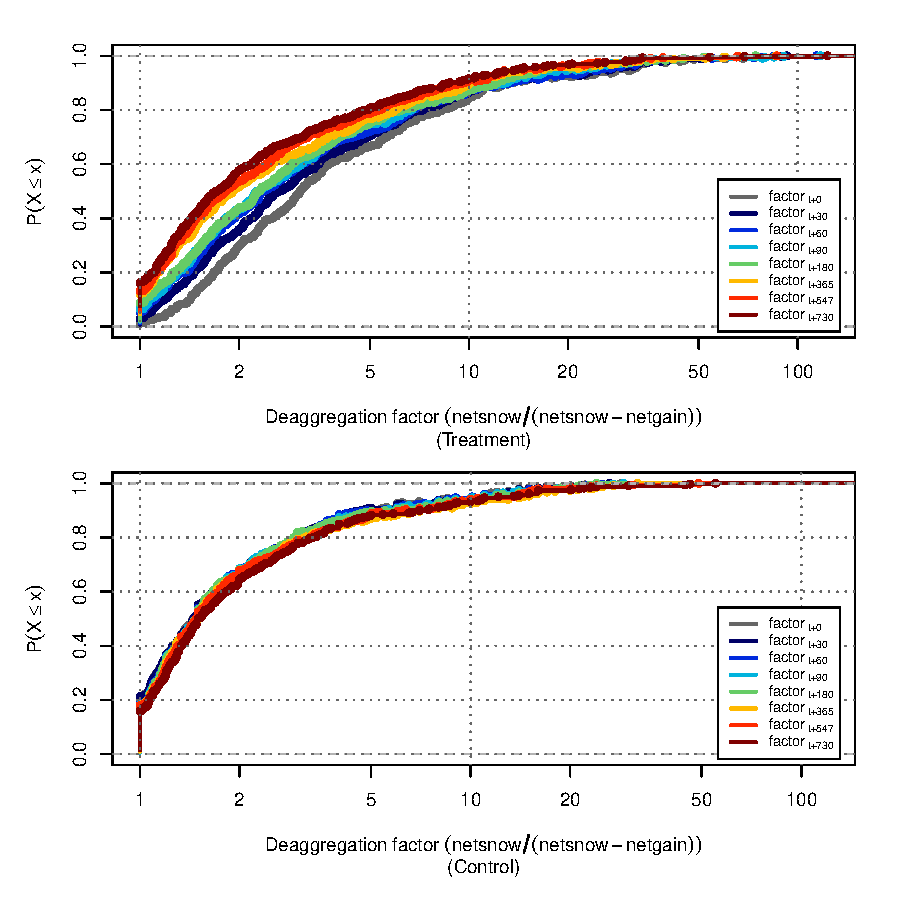
\includegraphics[width=6in]{figures/behavior-deagg_factor-1997_2011-corr.pdf}
    \vspace{-2em}\\
    \caption{Cumulative distribution function of change in the deaggregation
    factor, the ratio of currently advertised prefixes to perfectly aggregated
    prefixes, of treated and untreated (control) ASes, for the period
    1997--2011. This figure is for the entire period, instead of particular
    slots, and was included to be congruent with the full-period figures for
    other quantities included in the body of the thesis.}
\end{singlespace}
\end{centering}
\end{figure}

\begin{figure}[H]
\begin{centering}
\begin{singlespace}
    \includegraphics[width=6in]{figures/behavior-deagg_factor-1998_2001-corr.pdf}
    \vspace{-2em}\\
    \caption{Cumulative distribution function of change in the deaggregation factor, the ratio of currently advertised prefixes to perfectly aggregated prefixes, of treated and untreated (control) ASes, for the period 1998--2001.}
\end{singlespace}
\end{centering}
\end{figure}
\begin{figure}[H]
\begin{centering}
\begin{singlespace}
    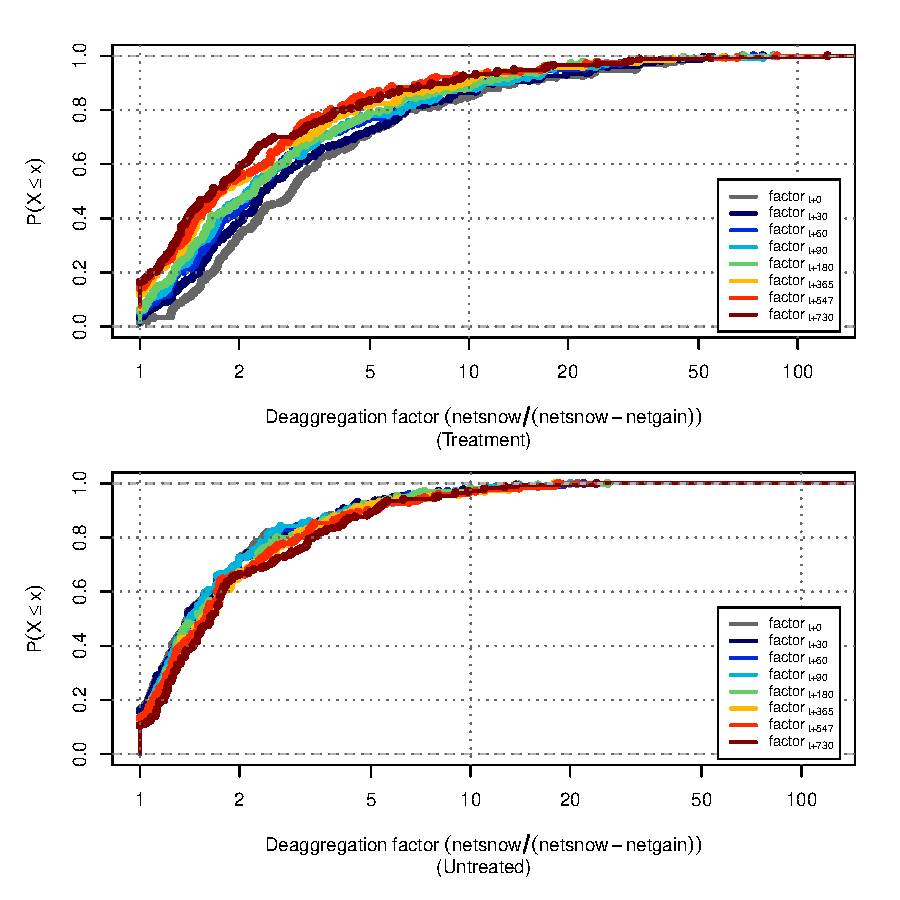
\includegraphics[width=6in]{figures/behavior-deagg_factor-2001_2004-corr.pdf}
    \vspace{-2em}\\
    \caption{Cumulative distribution function of change in the deaggregation factor, the ratio of currently advertised prefixes to perfectly aggregated prefixes, of treated and untreated (control) ASes, for the period 2001--2004.}
\end{singlespace}
\end{centering}
\end{figure}
\begin{figure}[H]
\begin{centering}
\begin{singlespace}
    \includegraphics[width=6in]{figures/behavior-deagg_factor-2004_2007-corr.pdf}
    \vspace{-2em}\\
    \caption{Cumulative distribution function of change in the deaggregation factor, the ratio of currently advertised prefixes to perfectly aggregated prefixes, of treated and untreated (control) ASes, for the period 2004--2007.}
\end{singlespace}
\end{centering}
\end{figure}
\begin{figure}[H]
\begin{centering}
\begin{singlespace}
    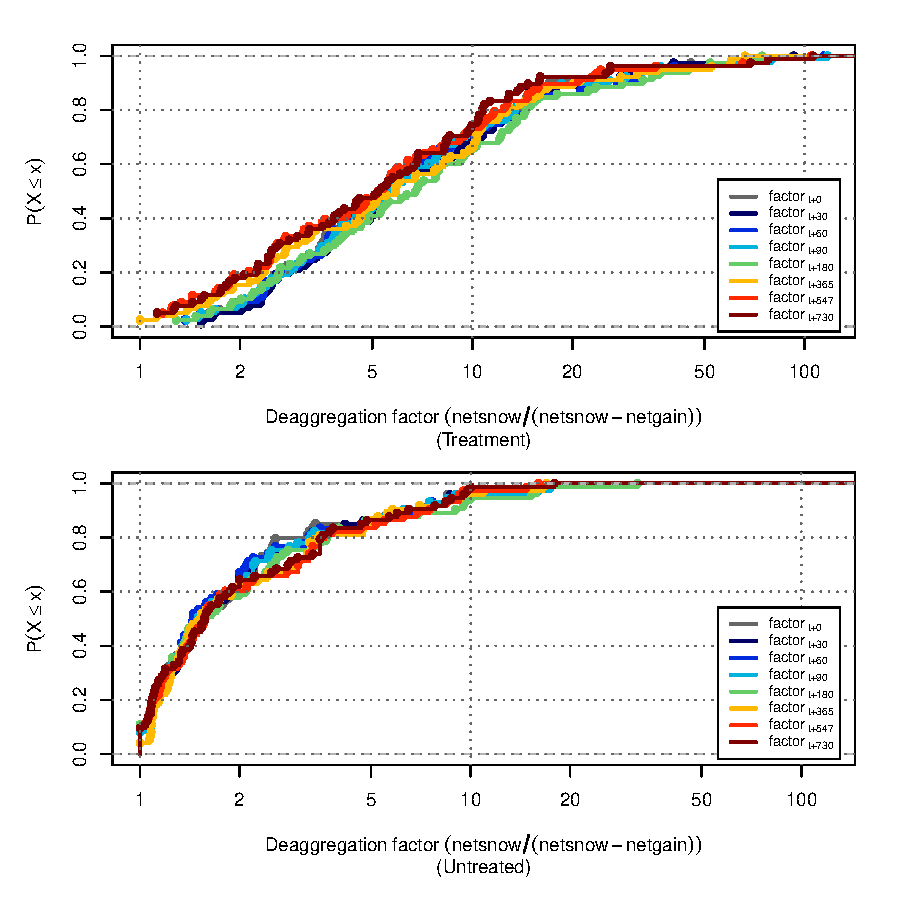
\includegraphics[width=6in]{figures/behavior-deagg_factor-2007_2010-corr.pdf}
    \vspace{-2em}\\
    \caption{Cumulative distribution function of change in the deaggregation factor, the ratio of currently advertised prefixes to perfectly aggregated prefixes, of treated and untreated (control) ASes, for the period 2007--2010.}
\end{singlespace}
\end{centering}
\end{figure}